	\subsection{Conceptos Fundamentales}
		\begin{itemize}
			\item Poblacion o Poblacion Objetivo: Conjunto de elementos sobre los que queremos hacer afirmaciones.
			\item Muestra: Subconjunto de la poblacion que se extrae para ser estudiado.
			\item Marco Muestral: Conjunto de elementos de la poblacion suceptible de ser muestreada.
		\end{itemize}
	\subsection{T\'ecnicas de Muestreo}
		\begin{itemize}
			\item Muestreo No-Aleatorizado (o No-probabilista): Se basa en el juicio personal del investigador. Puede generar buenas muestras pero no permite una evaluaci\'on de confianza.
			\item Muestreo Aleatorizado (o Probabilista): se controla la probabilidad de seleccionar un determinado individuo del marco muestral. Permite estudiar objetivamente la confianza de las generalizaciones hacia la poblaci\'on objetivo.
		\end{itemize}
		\textbf{?`Como recolectar los datos?}\\
		\begin{itemize}
			\item Muestreo no-Aleatorizado o no-Probabilistico
			\begin{itemize}
				\item Muestreo por conveniencia: Los elementos de la muestra se eligen por estar en el lugar o en el momento adecuado para la investigacio\'on. 
				\item Muestreo por juicio: Se selecciona de acuerdo a alguna caracter\'istica especifica del encuestado juzgada por el encuestador.
				\item Muestreo por cuota: Intenta mejorar la representatividad de la muestra separando a la poblaci\'on de acerdo a variables de control (edad, sexo, raza, ...). Luego a cada subgrupo se le asigna una cuota o proporci\'on de muestreo, t\'ipicamente \% de la poblacion.
				\item Muestreo tipo "bola de nieve": Se selecciona un grupo inicial. Luego, los nuevos encuestados se seleccionan en base a las referencias de los encuestados anteriores.
			\end{itemize}
			\item Muestreo Aleatorizado o Probabilistico
			\begin{itemize}
				\item Muestreo aleatorio simple: Cada elemento del marco muestral tiene la misma probabilidad de ser seleccionado y cada elemento se selecciona de manera independiente de los otros.
				 \begin{itemize}
					\item Con reemplazo: se pueden repetir elementos
					\item Sin reemplazo: no se pueden repetir elementos
				 \end{itemize}
				Se indeza a la poblacion y luego se elige un indice de manera aleatoria hasta completar el tama\~no deseado de la muestra.\\
				Generalmente se usa una tabla de numeros aleatorios.\\
				\item Muestreo sistematico: Se elige un elemento de partida aleatoriamente y el resto se elige en sucesi\'on hasta completar la muestra.\\
				Si n es el tama~no de la muestra y N el de la poblacion muestra se determina $ s = \frac{N}{n}$ , con piso.
				\item Muestreo estratificado: Antes de seleccionar los elementos, se agrupa la poblacion muestral en estratos de acuerdo a una variable importante. Dentro de cada estrato se puede proceder con Muestreo simple o sistematico.
				\item Muestreo clusterizado: Se divide a la poblacion en grupos lo m\'as homogeneos entre ellos y los mas heterogeneos internamente. Se seleccionan aleatoriamente los grupos a encuestar ya sea de manera simple o sistematica (Cada grupo se selecciona completamente: se toman todos sus elementos).
			\end{itemize}
		\end{itemize}
	\subsection{Tipos de Datos}
		\begin{itemize}
			\item Cuantitativos: operables aritm\'eticamente.
				\begin{itemize}
					\item Escala Intervalar: Tienen sentido las diferencias.
					\item Escala de Raz\'on: Tienen sentido los cuocientes.
					\item Discretos/Continuos.
				\end{itemize}
			\item Cualitativos
				\begin{itemize}
					\item Categoricos: Son solo nombres de referencia.
					\item Ordinales: Se pueden jerarquizar u ordenar.
				\end{itemize}
			\item Estructurados: formados por conjuntos de los anteriores. (Ej: grafos, matrices)
		\end{itemize}
	\subsection{Frecuencia}
		La frecuencia es el n\'umero de veces que un suceso se repite en la muestra. Llamaremos frecuencia relativa a la fracci\'on de veces que \'este aparece en la muestra.
	\subsection{Presentacion de los Datos}
		\begin{itemize}
			\item Datos Categ\'oricos: Usualmente se presenta la frecuencia con la que ocurre cada uno de los valores.(Ej: Diagramas de torta, de barras, ...)
			\item Datos Ordinales: Los diagramas de barras se suelen ordenar de acuerdo a la jerarqu\'ia natural de los valores posibles. (Ej: estratos economicos)
			\item Datos Cualitativos: Cuando son muchos es posible agruparlos en subconjuntos, pero generados en general por criterios no-estadisticos.
			\item Datos Cuantitativos: Tabligrama - El ultimo digito se expresa separado de los mas significativos.\\ \\
			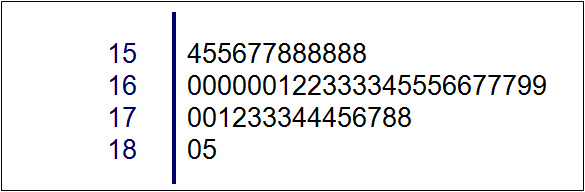
\includegraphics[scale=0.3]{images/tabligrama}
			\\ \\Tablas de frecuencias - Agrupar los valores en intervalos y registrar la frecuencia de ese grupo de valores en la muestra.\\
			Histograma - Los intervalos son todos del misma tama\~no y cubren uniformemente el rango de los datos.\\
			\begin{itemize}
				\item Rango = maximo - minimo
				\item Amplitud de cada clase: A = (Rango + 1)/K
				\item k-esimo intervalo: $[a_k,b_k] = [b_{k-1},b_{k-1}+A]  $
			\end{itemize}
		\end{itemize}
